\chapter{Technologies}
\thispagestyle{pagestyle}

Pie's technologies were chosen with maintainability in mind. I have integrated various technologies and third-party libraries already used in popular mature open-source projects. Such technologies are backed up by large communities and frequent updates, confirming that they will not become obsolete in the near future.

\section{Microsoft's Windows Forms and the .NET Framework}

THE .NET Framework was introduced in 2001 by Microsoft, together with the Visual Studio tool. It was built for the purpose to simplify Windows application development \cite{net-framework}, currently supporting three languages, also developed by Microsoft: Visual Basic, a user interface adaptation of the BASIC language, C\#, and F\#.

Pie uses Windows Forms (commonly referred to as "Winforms"), as the primary technology for its graphical user interface and business logic. Winforms is a technology that was introduced with the first version of .NET. It "can be thought of as a wrapper around the complex Win32 API" \cite{winforms-history}. The solution 
simplified desktop development by allowing programmers to focus on the business logic, instead of coding user interface components. Components, officially known as "Controls", could be added to application windows (or "Forms") simply by dragging and dropping them on the workbench.

Although not the first WYSIWYG ("What You See Is What You Get") designer, Windows Forms is certainly one of the most popular ones, as it came directly from Microsoft, the developer of Windows, receiving frequent updates and support even to this day. It is also available for all of the three .NET languages. I have chosen C\#, as it is the most commonly used among them.

Winforms is not the only user interface technology developed by Microsoft. Several years later, in 2006, Windows Presentation Foundations ("WPF") has been introduced, followed by the Universal Windows Platform ("UWP") technology in 2015. Although the latter provide a more actual way of splitting user interface logic and business logic, Windows Forms received more support during the years, is simpler to use, and has more compatible extensions ready to be integrated. Windows Forms is also considered to be a better option, from a memory management point of view. Performance is also a key to be taken into consideration, and in this manner, it seems that there is no significant difference between newer technologies such as WPF and Winforms \cite{han2023optimization}. Even so, the Form components inside Pie do not incorporate a large number of controls (e.g. buttons, textboxes, labels, panels) and the file handling logic is as simple and possible, using actual C\# integrated methods. Thus, the application is not expected to cause any slow-downs during the start-up or the usage of it.

The "Form" control is a representation of any window displayed in an application. The Form class can be used to create standard, floating and borderless windows. The "Properties" panel (present in any type of Control object), can be used to determine the appearance, size, color and window management features of the windows or dialog boxes that are created. \cite{form-class}

\begin{figure}[H]
\centering
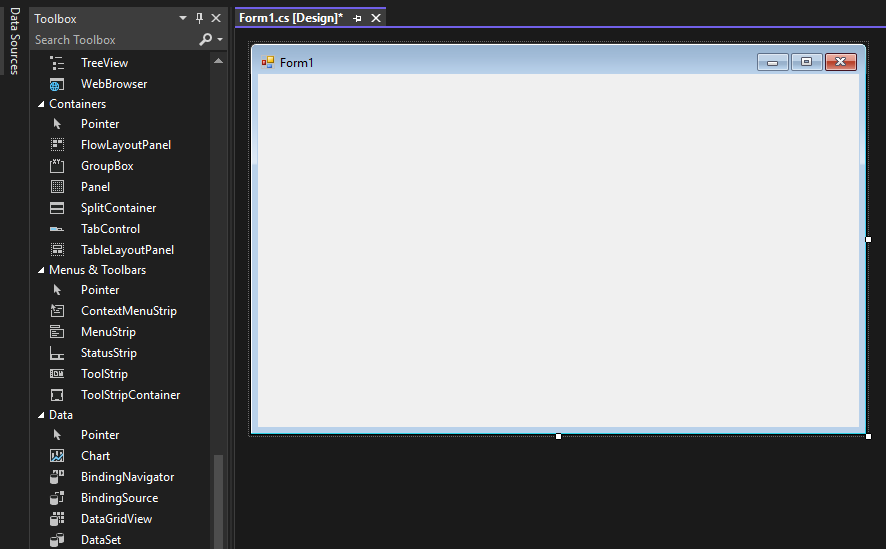
\includegraphics[width=0.8\textwidth]{images/winforms-designer.png}
\caption{Designing a Form using the Winforms technology in Visual Studio}
\label{fig:fig2,1.}
\end{figure}

Controls (available in the Toolbox sidebar of the designer) can have "Events" attached to them. Such events can be triggered on several occasions:

\begin{enumerate}
  \item a mouse is hovered over the control;
  \item the control is clicked;
  \item someone presses a key, while holding focus on the control. 
\end{enumerate}

Pie uses a large number of event handlers, in order to handle certain key bindings accordingly. By doing so, users can toggle different user interface components, such as the Find\&Replace dialog or the integrated terminal system, simply by pressing a combination of keys. 

The NuGet pacakge manager, integrated inside Visual Studio, is the most effective and secure way to add external libraries inside a .NET project. It provides a huge collection of packages built by developers, such as file parsers, user interface components or database drivers, ready to be bundled inside the application.

\begin{figure}[H]
\centering
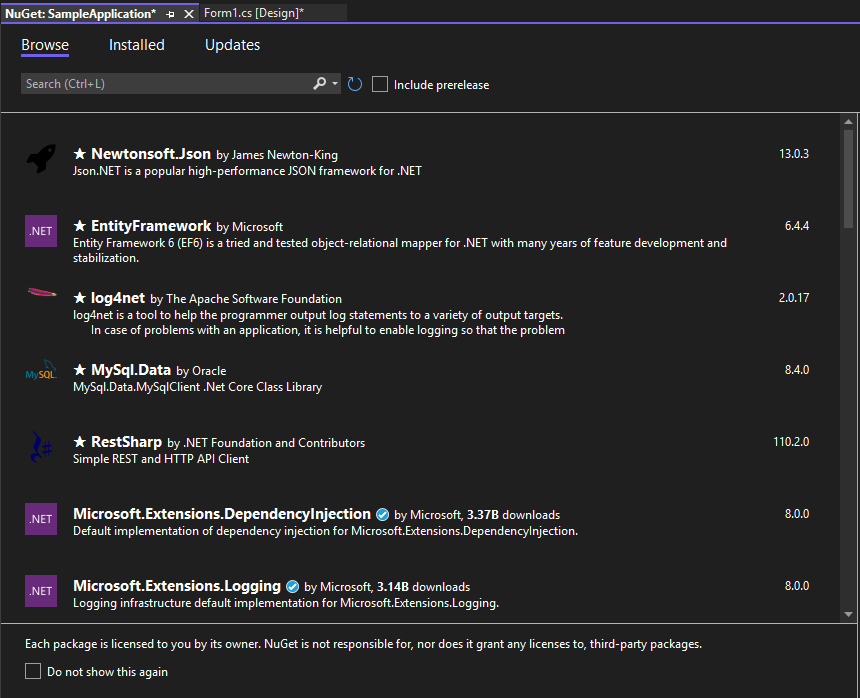
\includegraphics[width=0.8\textwidth]{images/nuget.png}
\caption{Using NuGet to discover packages available to install in a Windows Forms application}
\label{fig:fig2,1.}
\end{figure}

\section{Third-party libraries included with Pie}
\subsection{Redesigning .NET components with Krypton and ObjectListView}
\subsection{Relying on NewtonsoftJson to parse configuration files}
\subsection{Integrating the code editing functionality with Scintilla}
\subsection{Terminal instance management using ConEmu}
\subsection{Using CefSharp and Markdig for rendering code inside web browsers}
\subsection{Managing Git repositories with LibGit2}
\subsection{Querying databases with various SQL drivers}